\chapter{深層学習による病理画像の診断支援}
\label{chap_review}

病理画像をデジタルで保存することが始まったのは数十年前になる.これによって遠隔地でも診断することができるようになったり,情報を共有することができるようになり,複数の医師で診断しミスを防止するセカンド・オピニオンが容易になった.計算機科学の分野の側面ではデータを収集することができるようになり,研究が盛んに行われることになった.その後は,様々な病理データでより改良されたアルゴリズムの提案が行われている.

細胞組織の形態を観察するための病理染色ではヘマトキシリン・エオジン染色(HE染色)が一般的に用いられる.細胞核を青紫色に染色し,細胞質をピンク色に染色する.正常から異常に変化していくと,細胞核が過度に増殖したり,細胞質の形が崩れたりすることで,その特徴を機械学習によって精度よく検出するための研究が行われている.

これまでは,核の形やテキスチャーからパターンマッチングなどの画像処理によって腫瘍を検出する研究されてきたが,近年になって画像処理に大きなブレークスルーが起きたことをきっかけに,新しい手法で解析するようになってきた.そのブレークスルーがディープラーニングである.

\section{ニューラルネットワーク}
人間の脳にはニューロンと呼ばれる神経細胞が1000億個以上あり,それぞれが複数のニューロンと電気信号で情報を伝達している.また脳には電気信号を受け渡すシナプスという場所がある.ニューロンとシナプスで行われる演算を模倣したアルゴリズムを作ることができれば人間のような思考や認識をコンピュータを使って再現できると考えた.そのアルゴリズムがニューラルネットワーク(Neural Network: NN)である.


\subsection{多層パーセプトロン}
ニューラルネットワークは入力層,出力層,隠れ層から構成され,層と層の間にはニューロン同士のつながりの強さを示す重みがある.非線形問題を扱うために1986年Rumelhartによって考案されたのが,パーセプトロンを複数つなぎ合わせ入力と出力以外に隠れた層を持つ多層パーセプトロン(Multi-layer perceptron: MLP)である(\fig {mlp}).ニューラルネットワークで多層パーセプトロンの層を全結合(fully connected: FC)層とも呼ぶ.
\begin{figure}
	\centering
	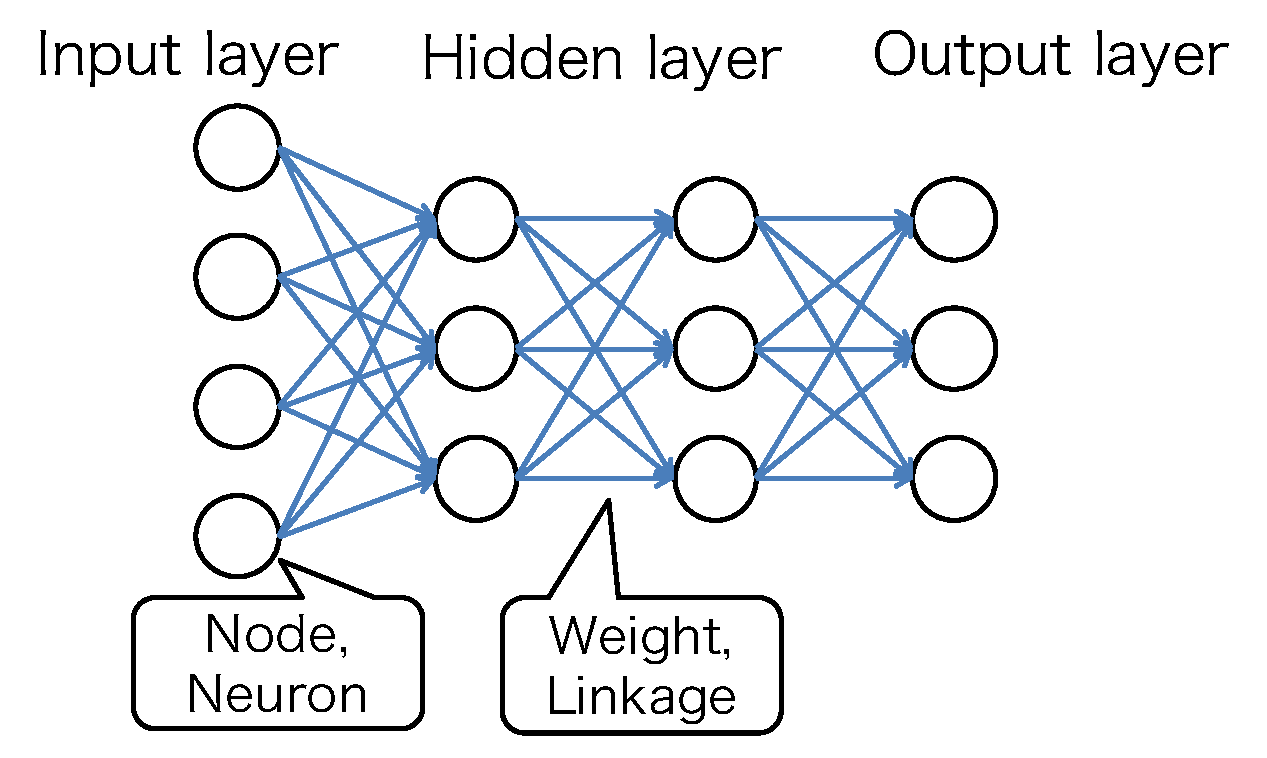
\includegraphics[width=0.7\linewidth]{fig/MLP}
	\caption{Architecture of Muti-layer perceptron}
	\label{fig:mlp}
\end{figure}
\fig {mlp}における丸や矢印はそれぞれノード(またはニューロン)と重み(または結合)と呼び,ともに数値である.例えば画像を分類しようと思えば,各ピクセルの画素数を各ノードに入力する($28 \times 28$pixelのグレースケール画像であれば784個のノードが必要).データが入力層に入ってくると,その値に重みをかけ,活性化関数と呼ばれる関数を通し結果を出力する.これを繰り返し出力層に書き出す.各層の重みの値によって出力結果は異なってくる.出力層のノードは区別したいクラス数分用意し,各ノードの出力値が各クラスに属している確率を表す.

学習については誤差逆伝播法を利用する.ニューラルネットワークの出力値と正解データとの比較をした時に,どれだけ正解から離れているかを評価する損失関数(Loss function)を使って,損失関数が小さくなるようにノード間の重みを勾配降下法によって更新する.


\subsection{畳み込みニューラルネットワーク}
畳み込みニューラルネットワーク(Convolutional Neural Network: CNN)は,1998年には既にLeNetと呼ばれるネットワークで実装されていた\cite{LeNet}.Deep Learning元年が2012年であることを考えるととても驚きである.
\begin{figure}
	\centering
	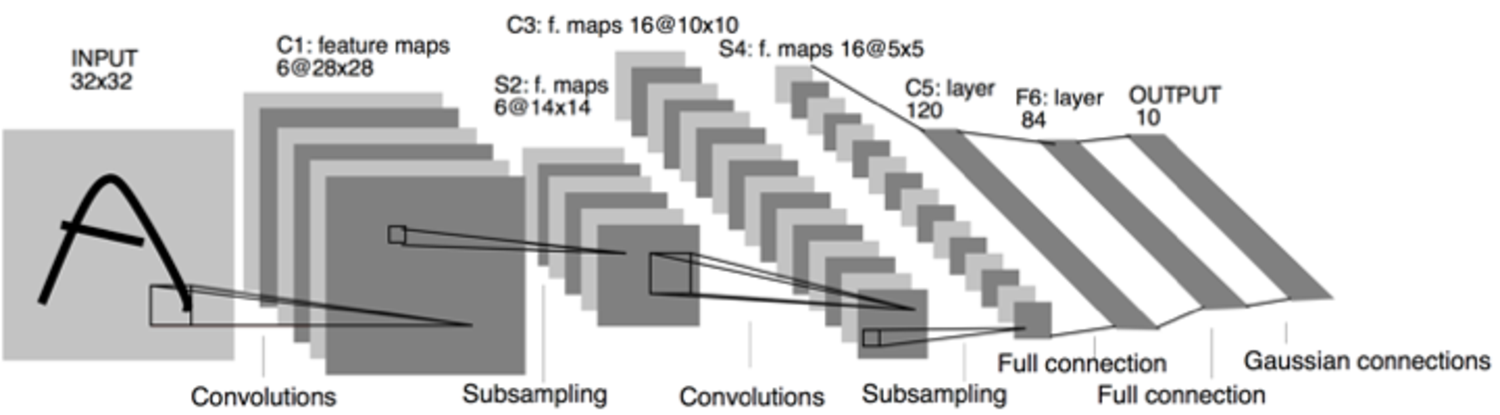
\includegraphics[width=0.7\linewidth]{fig/LeNet}
	\caption{Architecture of convolutional neural network\cite{LeNet}}
	\label{fig:LeNet}
\end{figure}
従来の画像認識では,画像から特徴を抽出し,それをニューラルネットワークにかけるいわゆる特徴量設計が必要で,ここをいかにうまく設計するかがポイントであったが,CNNは特徴量設計から識別までをend-to-endで行うことがきることが最大の強みである.人間が物体を認識することをコンピュータにも計算させるには,画像の特徴的な部分を切り分けて数値化させる必要がある.例えば,カラー画像の場合,RGBの3色(3チャンネル)を組み合わせた画像で認識をしている.このようなフィルターの畳み込み計算を行うと,フィルターごとに異なった画像の特徴を抽出して数値化する.これが畳み込み(convolution)である.その後,画像のサイズを小さくしてコンピュータが計算コストを減らし,微小な変化に対してロバストになる仕組みしてプーリングという方法を用いる.学習にはMLPと同様に誤差逆伝播法を用いる.


\subsection{再帰的ニューラルネットワーク}
再帰的ニューラルネットワーク(Recurrent Neural Network: RNN)は時系列解析や自然言語処理に利用されるニューラルネットワークである.内部にループを持つことで過去の情報を保持しておくことができる.
時系列の入力 $x = (x_1, \cdots , x_T)$ があった時に,出力 $y = (y_1, \cdots , y_T)$と隠れ層のベクトル $h = (h1, \cdots ,h_T)$をそれぞれ以下の式で計算する.

\begin{align}
\label{eq:RNN}
  h_t & = H(W_{ih} x_t + W_{hh} h_{t-1} + b_h) \\ 
  y_t & = W_{ho} h_t + b_o
\end{align}

$W$は重みの行列であり($W_{ih}$は入力と隠れ層間の重み行列),$b$はバイアス項である.そして$H$が活性化関数である.

RNNは過去の情報をどこまでさかのぼって関連性を見つけるかを判断することができないため,時系列データが長くなるほど,その長期の依存性を学習するには人が慎重にパラメータを設計する必要があるなど,学習が難しくなるという問題があった.この問題を解決するためにLong-short term memory(LSTM)が提案された.LSTMもRNNの一種であるため繰り返し構造を持ち,3つのゲートを持つ層からなっている. 

\begin{figure}[h]
\centering
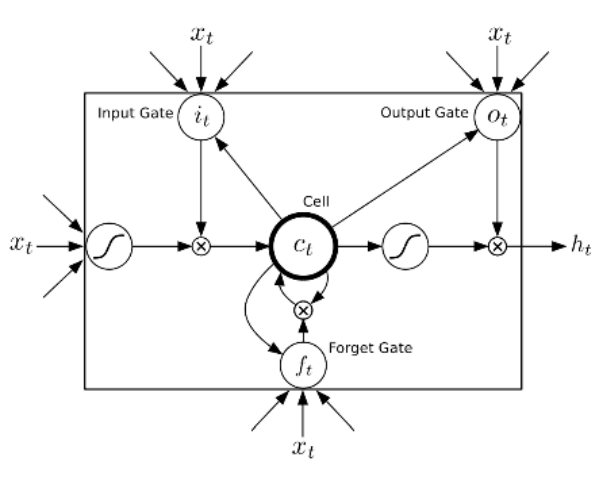
\includegraphics[width=0.7\linewidth]{fig/lstm.png}
\caption{}
\label{fig:LSTM}
\end{figure}

\begin{align}\label{eq:LSTM}
  f_t & = \sigma(W_{xf} x_t + W_{hf} h_{t-1} + W_{cf} c_{t-1} + b_f ) \\
  i_t & = \sigma(W_{xi} x_t + W_{hi} h_{t-1} + W_{ci} c_{t-1} + b_i) \\
  c_t & = f_t c_{t-1} + i_t \tanh(W_{xc} x_t + W_{hc} h_{t-1} + b_c) \\
  o_t & = \sigma(W_{xo} x_t + W_{ho} h_{t-1} + W_{co} c_t + b_o) \\
  h_t & = o_t \tanh(c_t) 
\end{align}

ここで$\sigma$はシグモイド関数であり,次の式で定義される.
\begin{equation}\label{eq:sigmoid}
  \sigma (x) = \dfrac{1}{1 + e^{-x}}
\end{equation}

$f_t$で示される層は忘却ゲート層と呼ばれ,過去の情報で捨てるべき情報を判断する.これはシグモイド層によって行われ,0と1の間の値を出力し,0は完全に忘れる.1は完全に維持するという意味である.
$i_t$や$c_t$で示される層は,入力ゲート層と呼ばれ,$i_t$で新たに入力された情報から,どの情報を更新するかを判断し$c_t$で古い情報を落とし新しい情報を加え,値を更新する.
最後が$o_t$や$h_t$で示される層で,出力ゲート層と呼ばれる.まず何を出力するべきかを$o_t$のゲートで判断して,$c_t$に$\tanh$を適用して掛けることで出力が計算される.

\section{推論と学習}
ニューラルネットワークでは推論フェーズと学習フェーズに分かれている.
誤差逆伝播法


\section{画像認識におけるディープラーニング}
%教師あり学習であることもここで触れておきたい
Deep LearningとはDeep Neural Network(DNN)を指すことが多い.この"Deep"とは,ニューラルネットワークの層が深いことに由来している.

\fig {ImageNet}に画像認識タスクの精度の近年の推移を示す.これはImageNet Large Scale Visual Recognition Challenge (ILSVRC)と呼ばれる世界的な画像認識のコンペティションである(2010年から始まった).カテゴリ数は1000クラスで,画像枚数は120万枚の訓練データと15万枚のテストデータが用意されている.
\begin{figure}
	\centering
	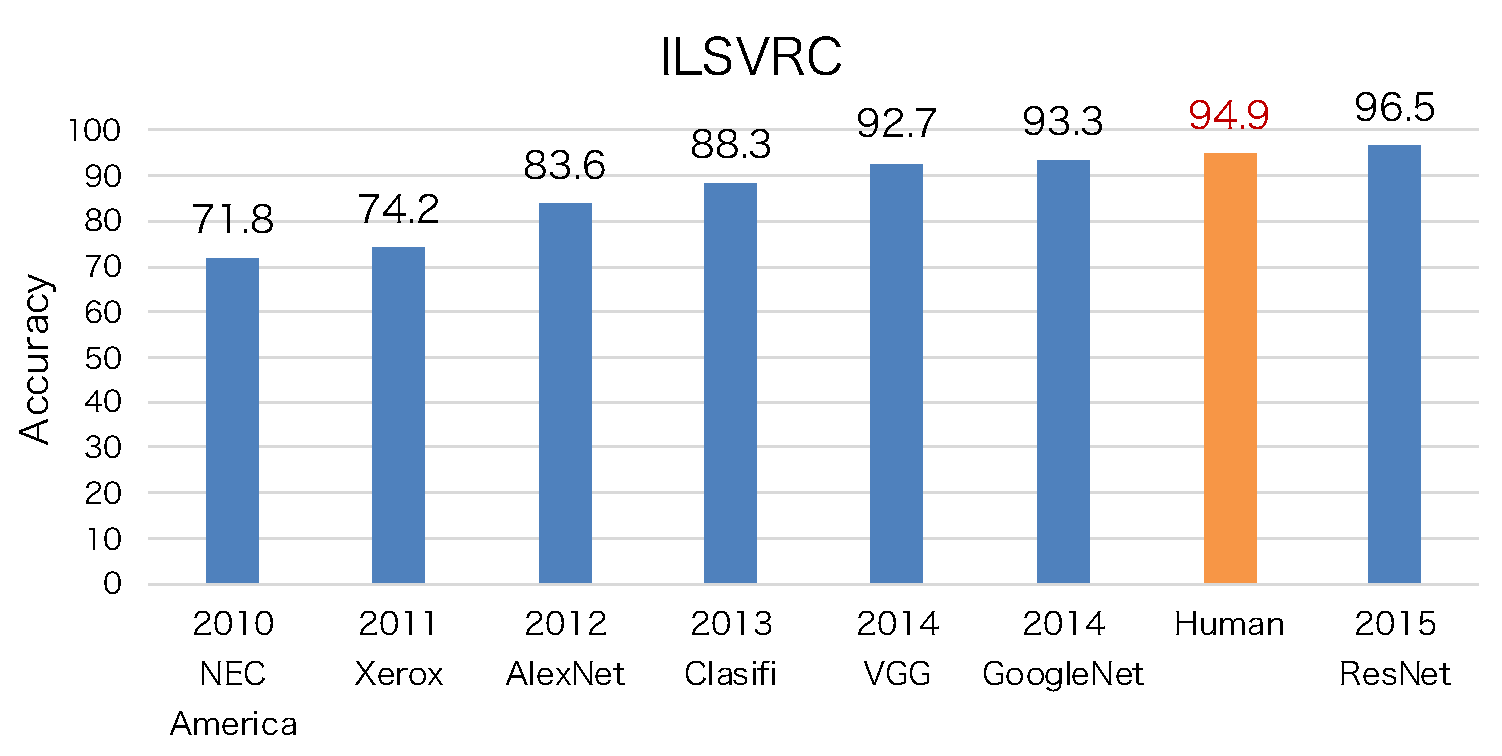
\includegraphics[width=0.7\linewidth]{fig/ILSVRC}
	\caption{Transition of accuracy of image recognition on ILSVRC}
	\label{fig:ImageNet}
\end{figure}
2011年と2012年は約10\%もの大差でAlexNet\cite{AlexNet}が優勝している.これがディープラーニングの始まりである.AlexNetは5つの畳み込み層と3つの全結合層を持っている.2014年にはVGGNet\cite{VGGNet}やGoogLeNet\cite{GoogLeNet}が9割の精度を超えた.VGGNetはAlexNet(8層)よりさらに深い構造(19層)であり,GoogLeNetは22層もある.そして2015年にはResNet\cite{ResNet}が人間の精度をも超える認識精度を達成した.ResNetはGoogLeNetよりもさらに深く152層もある.CNNを複数回かけて検出を行う場合,CNNの浅い側では空間分解能はあるが抽象的な情報が少ない.深い側では意味論的な情報は取得できる(ポーズ,変形など)が空間分解能が小さいため幾何学的な情報が失われる.

アーキテクチャの進化の方向は大きく3つある.1つ目は層を深くすることである.
2つ目はFC層の使用を避ける,またはInceptionモジュールの使用することである.これにより学習するパラメータ数を削減することができる.3つ目はResNetなどのショートカット接続の利用や,事前学習・転移学習を行うことである.これによって学習効率を向上させ,最終的にモデルの精度向上へと繋がる.ここで,事前学習のデータセットと適用データとの間には類似性があると良い.


画像処理におけるディープラーニングでは大きく3つのタスクがあり,それぞれ,クラス分類,物体検出,セグメンテーションである.以下に詳細を述べる.

\subsection*{クラス分類}
カテゴリ分けをすること

\subsection*{物体検出}
物体検出とはBounding Boxで物体の位置とその物体の種類を特定する方法である.歴史的には幾何的情報,手動特徴量,そしてそのカスケードを利用していた.その後,HOGやSIFTなど局所特徴量を抽出する方法を設計するようになったが,これは深い専門知識を必要とした.また広い範囲でオブジェクトを正確に検出する方法は,メモリ容量と処理時間に課題がある.現在はDeep Neural Networkになりデータのみから抽象的な特徴量を複数得ることができる.一般物体認識の場合は数千のカテゴリを学習してTop Error Rateが2\%以下と人間よりも認識精度が高いが,物体検出においては,今はカテゴリがせいぜい数百程度くらいまででも認識精度が人間よりも低くなってしまう.また物体検出は精度を上げるために処理に時間がかかるアルゴリズムであることが多いため,リアルタイムに物体検出を行う時は,速度と精度でトレードオフが生じてしまう.

\begin{figure}[h]
\centering
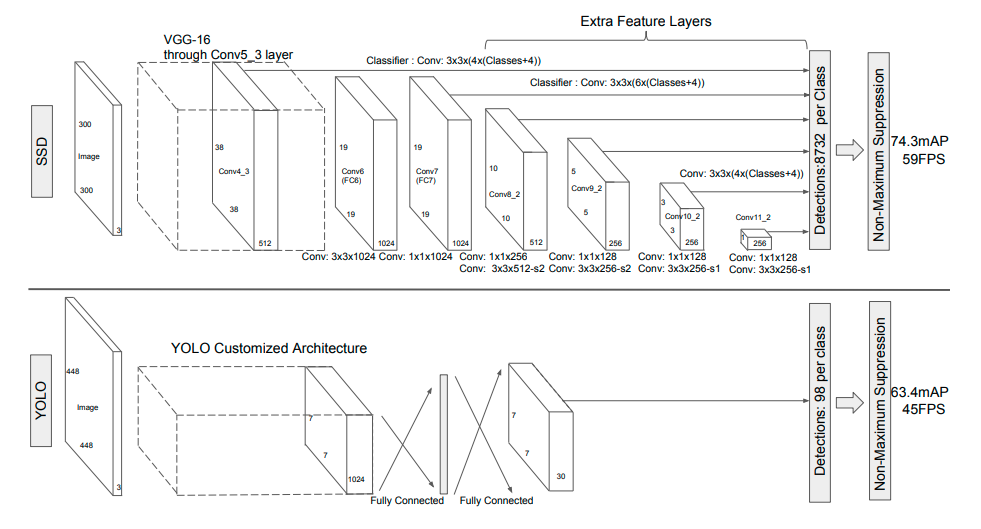
\includegraphics[width=0.7\linewidth]{fig/yolo_ssd.png}
\caption{Network Architecture of SSD and YOLO}
\label{fig:YOLO}
\end{figure}

\subsection*{セグメンテーション}
セマンティックセグメンテーションとは,画像を画素レベルで認識することである.画像内の各画素をオブジェクトクラスに割り当てる手法である.セマンティックセグメンテーションの手法についてディープラーニング以前では,Texton Forestsや,Random Forestsに基づいた分類を行っていたが,物体検出と同様にCNNが登場してからは,高精度なセグメンテーションが実現するようになった.CNNを使ったセグメンテーションの手法で一般的に使われるようになったものがUnetである(\fig {Unet}).このUnetは文字通りUの形をしたネットワークであることが特徴で,2つのアーキテクチャーからできている.1つ目がエンコーダーのアーキテクチャーでCNNとプーリングで特徴を抽出しながら次元を削減していき,2つ目のデコーダーのアーキテクチャーで画像をセグメンテーションの結果になるように復元する.ここで問題になることが,プーリングをすることで位置情報を消してしまっているので,この位置情報を利用して画像を復元するためには,エンコーダーとデコーダーで画像サイズが同じところ同士をショートカットで接続することがUnet構造の優れている点である.

\begin{figure}[h]
\centering
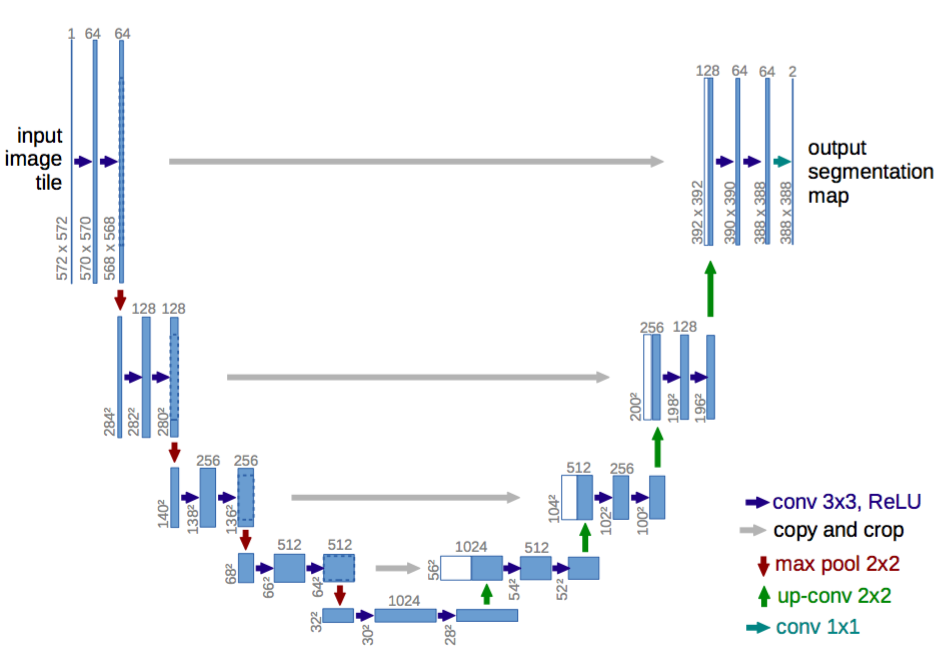
\includegraphics[width=0.7\linewidth]{fig/unet.png}
\caption{}
\label{fig:Unet}
\end{figure}

\section{深層学習による3次元画像解析}
ディープラーニングを医療画像に応用するコンペティションが世界で行われているが,その半数が3D医療画像の解析になっているほど需要が高まっている.その理由は,現在解決しなくてはならない課題があるからである.まずは2次元画像と違って,処理するべきデータが大きいということである.そのため学習するパラメータをなるべく少なくする工夫がされている.また3次元画像には,動画または,ボリューム画像があるが,2次元画像とその深さ方向(動画であれば,時間方向)には異方性があることから,機械学習の方法に工夫が必要になる.今まで考案されている手法として,2DCNNを拡張した3DCNN,またCNNと時系列解析でよく用いられるLSTMを組み合わせた手法と,LSTM内部にCNNを組み込んだ手法,それらをすべて組み合わせた手法が考案されいる.LSTMの研究も盛んに行われているため,その改良モデルが数多く存在する.特に,LSTMの学習効率を上げたGRU(Gated Linear Unit)や,順方向だけでなく逆方向の時系列も計算に入れるBiLSTMが時系列解析の精度向上になっている報告がある.


\subsection{3DCNNとStacked Convolution}
2次元画像が深さ方向に連続している3次元画像の特徴を抽出するために,2次元のCNNを拡張して,3次元のカーネルを使って畳み込みを行う,3DCNNを利用した手法がある.

\begin{figure}[h]
\centering
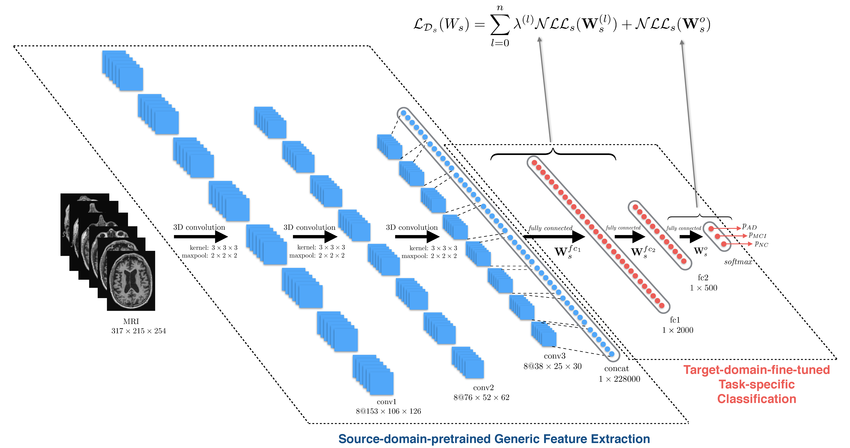
\includegraphics[width=0.7\linewidth]{fig/3d_cnn.png}
\caption{}
\label{fig:}
\end{figure}


\begin{figure}[h]
\centering
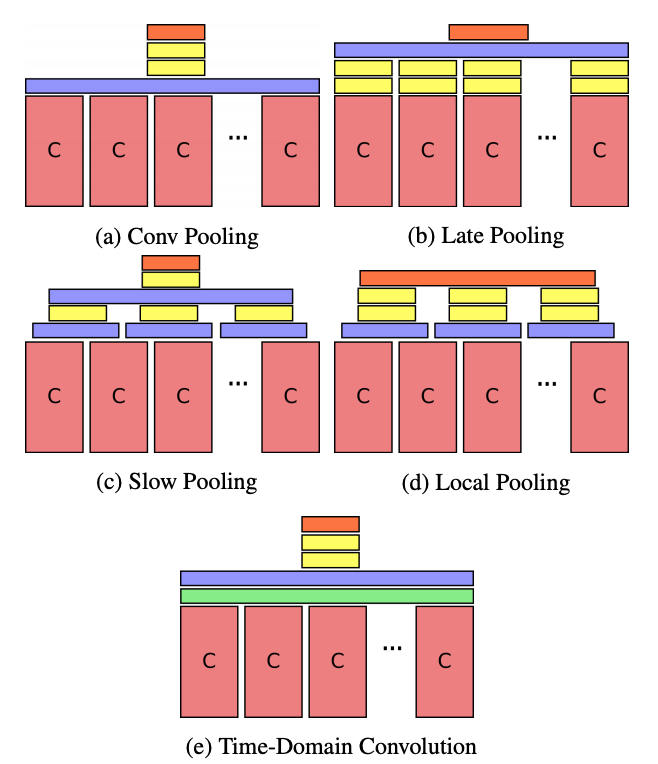
\includegraphics[width=0.7\linewidth]{fig/stacked_conv.png}
\caption{}
\label{fig:}
\end{figure}

\subsection{LSTMと2DCNNの組み合わせ}
時系列解析に使われるLSTMを用いて3次元の画像を解析することができる.これはよく動画の解析で行われることがある.つまりフレームごとの画像の特徴を2次元のCNNで計算してから時系列情報をLSTMで解析することで,画像の時系列解析を行うことができる.これを3次元の医療画像でCTやMRIで適用する研究も行われている.3DCNNのデメリットであったパラメータの増大を2DCNNとLSTMの組み合わせで解決することができる.

\section{教師なし学習}
機械学習の手法には,上記で説明したように,ラベルの貼られているデータセットを用いて学習することを教師あり学習と呼び,その反対で,データセットはあっても,そのデータセットの特性を示したラベルが与えられていない場合のデータセットを用いて学習することを教師なし学習と呼ぶ.

\subsection{Autoencoder}
教師なし学習で画像の特徴を抽出する方法としてオートエンコーダがある.画像の場合におけるオートエンコーダの手法とは,ある画像から情報を圧縮する「エンコーダ」と言われる部分と,その圧縮した情報から画像を復元する「デコーダ」の二つからなる.入力とデコーダから復元された画像が同じ画像になるようにニューラルネットワークで学習させる.この学習の結果,潜在変数は似てる画像どうしで近い値になるように変化し,この分布を見れば画像の分類を教師ラベルがなくても,学習を行うことができる.

\subsection{Variational Autoencoder}
本研究では,このオートエンコーダの派生である.Variational Autoencoder(VAE)を利用した.これはオートエンコーダの「エンコーダ」と「デコーダ」は同じネットワーク構造であるが,データセットの潜在変数の分布が,正規分布になるような制約を加えて学習を行う手法である.こうすることでAutoencoderの潜在変数では分布の距離に意味ないが,VAEでは正規分布に埋め込まれるため,画像の類似度を分布が表現することができるところが特徴である.

\subsection{敵対的生成ネットワーク}
敵対的生成ネットワーク(Generative Advarsarial Network: GAN)は2014年に提案された手法である.\fig {GAN}のようにGANではGeneratorとDiscriminatorの2つのネットワークがある.Generatorは訓練データと同じような画像を生成するネットワークでDiscriminatorは,入力されたデータが訓練データから来たものかGeneratorで生成されたものかを識別するように学習する.
VAEよりもGANの方が細部まで鮮明に画像を生成することができる.しかしGANは計算時間がかかるという問題や,DiscriminatorかGeneratorのどちらかか強くなってしまうなど,学習が安定しない問題があるため,これについての多くの研究報告がされている.

\begin{figure}[h]
\centering
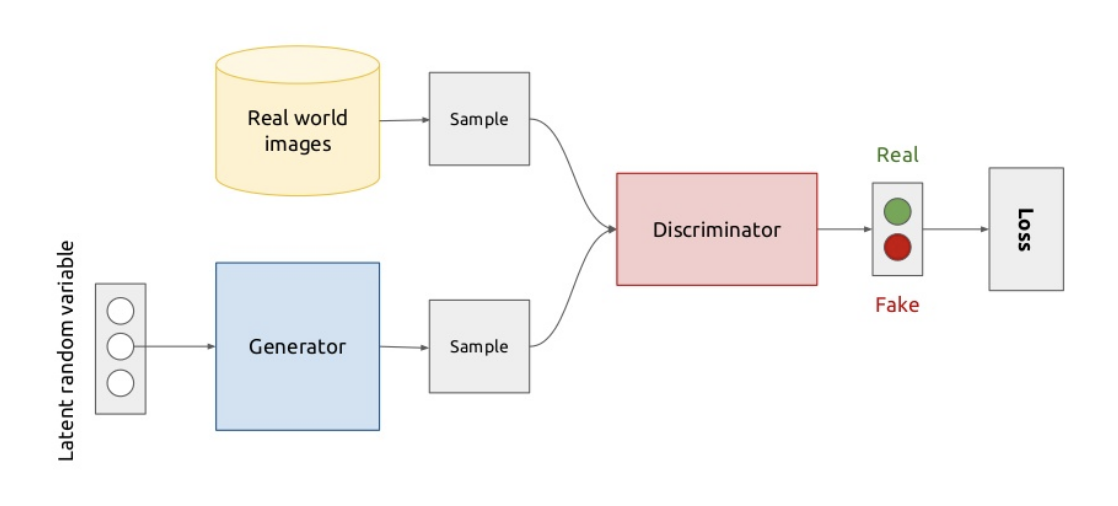
\includegraphics[width=0.7\linewidth]{fig/generative_adversarial_nets.png}
\caption{}
\label{fig:GAN}
\end{figure}

\section{半教師あり学習}
弱教師あり学習とも呼ばれる.これは,教師あり学習と教師なし学習を組み合わせて学習する方法である.こうすることでデータに教師ラベルをつけているものが少数であっても,データの特徴を学習しながら少量のラベルで識別境界を決めることができる.
GANやVAEの考え方を発展させてネットワークを構築することが考えられる.
